%%%%%%%%%%%%%%%%%%%%%%%%%%%%%%%%%%%%%%%%%
% FRI Data Science_report LaTeX Template
% Version 1.0 (28/1/2020)
%
% Jure Demšar (jure.demsar@fri.uni-lj.si)
%
% Based on MicromouseSymp article template by:
% Mathias Legrand (legrand.mathias@gmail.com)
% With extensive modifications by:
% Antonio Valente (antonio.luis.valente@gmail.com)
%
% License:
% CC BY-NC-SA 3.0 (http://creativecommons.org/licenses/by-nc-sa/3.0/)
%
%%%%%%%%%%%%%%%%%%%%%%%%%%%%%%%%%%%%%%%%%


%----------------------------------------------------------------------------------------
%	PACKAGES AND OTHER DOCUMENT CONFIGURATIONS
%----------------------------------------------------------------------------------------
\documentclass[fleqn,moreauthors,10pt]{ds_report}
\usepackage[english]{babel}
\usepackage{float}
\graphicspath{{fig/}}




%----------------------------------------------------------------------------------------
%	ARTICLE INFORMATION
%----------------------------------------------------------------------------------------

% Header
\JournalInfo{UL FRI Data Science - Introduction to Data Science, 2021-2022}

% Interim or final report
\Archive{Interim report}
%\Archive{Project X Report}

% Article title
\PaperTitle{Product recommendation system}

% Authors and their info
%\Authors{David Ocepek, Klementina Pirc, Matej Miočić\textsuperscript{1}}
%\affiliation{\textsuperscript{1}\textit{mm9520@student.uni-lj.si, 63180206}}

% Multiple authors
\Authors{David Ocepek\textsuperscript{1}, Klementina Pirc\textsuperscript{2} and Matej Miočić\textsuperscript{3}}
\affiliation{\textsuperscript{1}\textit{do8572@student.uni-lj.si, 63160248}}
\affiliation{\textsuperscript{2}\textit{kp3437@student.uni-lj.si, 63210492}}
\affiliation{\textsuperscript{3}\textit{mm9520@student.uni-lj.si, 63180206}}

% Keywords
\Keywords{recommendation system, products, RankFM, DeepFM}
\newcommand{\keywordname}{Keywords}


%----------------------------------------------------------------------------------------
%	ABSTRACT
%----------------------------------------------------------------------------------------

\Abstract{
For our project we have evaluated two models FM and deepFM using seen and unseen products.
The best performing model was FM with a Top-5 hit rate of 0.64 outperforming the baseline of 0.44, while deepFM scored 0.24.
On unseen products FM had a Top-5 hit rate of 0.23, in comparison to the baseline of 0.20, while we did not evaluate deepFM due to its poor performance.
Our model enables Siemens to feature ads that match the interests of 2-in-3 customers for old products.
and 1-in-4 for newly launched products.
}

%----------------------------------------------------------------------------------------

\begin{document}

% Makes all text pages the same height
\flushbottom

% Print the title and abstract box
\maketitle

% Removes page numbering from the first page
\thispagestyle{empty}

%----------------------------------------------------------------------------------------
%	ARTICLE CONTENTS
%----------------------------------------------------------------------------------------

\section*{Introduction}
Sales performance is one of the most important aspects of businesses therefore a lot of effort goes into its advancement. Suggesting new popular products to customers or products adjusted to their needs contributes to mentioned goals and this is where recommendation systems are utilised. Our goal was to create a recommendation system for Siemens which provided us with information about their customers purchases. For the task we resorted to different models and we present our results below.

\vspace{-0.3cm}

%------------------------------------------------

\section*{Data analysis}

Our data set consists of 1249 consecutive days for which we have information about sales for each customer. Starting date is unknown and purchase amounts are scaled down. \textit{5HB8\_4N50\_1I6D} is an example of a product label, where \textit{5HB8} is the family, \textit{4N50} the product and \textit{1I6D} product's variation. Data set contains 2762 customers, 126 families, 2013 products and 12304 variations.

\begin{figure}[hbt]\centering
	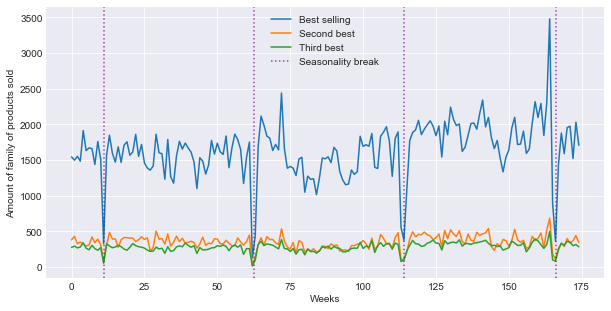
\includegraphics[width=\linewidth]{top products.png}
	\caption{Amount of \textbf{top 3 families of products} sold by weeks and a recurring seasonality break of drop in sales.}
	\label{top}
\end{figure}

\noindent We show the dominance of the most popular family of products in Figure \ref{top}, by comparing amount of sales to the second and third most popular family of products. We observe that the most popular family has approximately three times as much sales as the second best. Meanwhile sales of second and third best are more similar. We also observe a seasonality break that recurs every year.

\noindent To better understand the diversity of purchases we explore the number of unique variations, products and families for each customer. Results are shown in Figure \ref{unique} and we see that most customers bought only a small number of different products.

\begin{figure}[H]\centering
	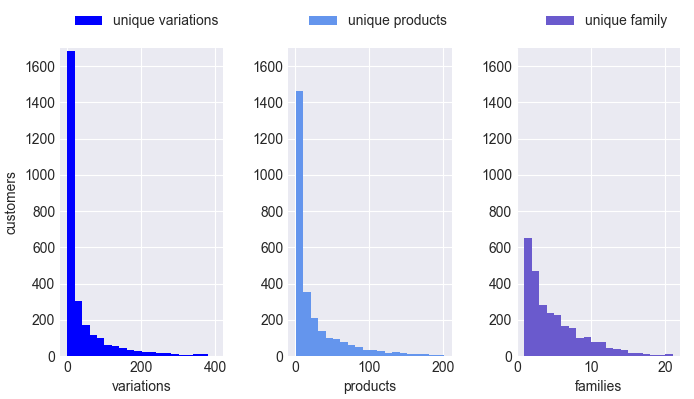
\includegraphics[width=\linewidth]{unique.png}
	\caption{Distribution of unique families, products and variations per customer.}
	\label{unique}
\end{figure}

\section*{Methods}

\subsection*{Walk-forward cross-validation}

\noindent We are working with a time series data and the model must not learn from the future data, so the more general cross-validation techniques are not correct. Therefore we decided to use walk-forward cross-validation which is a technique that splits the data into folds but still preserves the data order. We decided to use 500 days as train data and 125 days as test data as it allows us to go through all the data in 6 folds (Figure \ref{cv}). 

\begin{figure}[H]\centering
	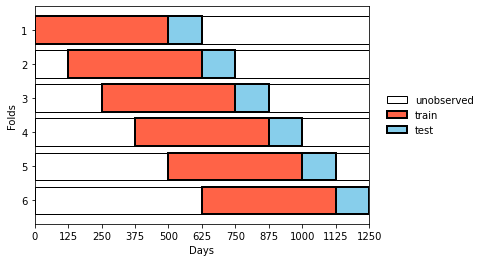
\includegraphics[width=\linewidth]{cv.png}
	\caption{\textbf{Walk-forward cross-validation.} We show how data is distributed into train and test data in consecutive folds.}
	\label{cv}
\end{figure}

\subsection*{Baseline}
Baseline model is important for understanding the true performance of our models. Baseline values for predictions are calculated by picking the most frequent family for each customer, then predicting top 5 variations or products from this family and finally checking if the customer bought any of them in the future. Family prediction is done independent of customers by always using top 5 families from the train set.

\subsection*{RankFM}

Factorization Machines (FM) are generic supervised learning models that map arbitrary real-valued features into a low-dimensional latent factor space and can be applied naturally to a wide variety of prediction tasks including regression, classification, and ranking. FMs can estimate model parameters accurately under very sparse data and train with linear complexity, allowing them to scale to very large data sets — these characteristics make FMs an ideal fit for real-world recommendation problems. \cite{fm}

RankFM\footnote{\url{https://github.com/etlundquist/rankfm}} is a python implementation of the general Factorization Machines model class adapted for collaborative filtering recommendation/ranking problems with implicit feedback user/item interaction data. This means we are not able to utilize explicit data such as the exact day and the amount of items purchased.

\pagebreak
\subsection*{DeepFM}

Deep Factorization Machines (DeepFM) is a family of supervised machine learning models combining neural networks (NN) and FM.
The main benefit DeepFM has over FM is its ability to model higher-degree non-linear interactions.
Additionaly, deepFM can use any type of NN such as LSTM or CNN~\cite{deepfm}.

DeepFM\footnote{\url{https://github.com/maciejkula/spotlight}} is a pytorch library implementing implicit and explicit models. 
For our task we used LSTM-FM with implicit negative sampling.
We tuned our models hyperparameters using Bayesian Optimization.

\section*{Results}

\begin{table}[H]
    \centering
    \begin{tabular}{c | c c c}
         & Baseline & RankFM & DeepFM  \\
         \hline
         Variation & 0.44 & 0.64 & 0.23 \\
         Product & 0.53 & 0.74 & 0.59 \\
         Family & 0.94 & 0.97 & -
    \end{tabular}
    \caption{Table showing top 5 hit rate for predicting \textbf{any} variations, products and families.}
    \label{popular}
\end{table}

\begin{table}[H]
    \centering
    \begin{tabular}{c | c c c}
         & Baseline & RankFM & DeepFM  \\
         \hline
         Variation & 0.20 & 0.23 & - \\
         Product & 0.22 & 0.31 & - \\
         Family & 0.24 & 0.26 & -
    \end{tabular}
    \caption{Table showing top 5 hit rate for predicting \textbf{only new} variations, products and families.}
    \label{popular_new}
\end{table}
From our results we conclude that Siemens can recommend ads users are interesting with fairly high likelihood.
The prior is partially due to Siemens customer tendencie of buying the same goods over-and-over again.
%------------------------------------------------

\section*{Discussion}

DeepFM performed very poorly and further analysis is neccesary to conclude whether this failure was because of a coding error or a specific failure of the deepFM model.


%------------------------------------------------

%\section*{Acknowledgments}


%----------------------------------------------------------------------------------------
%	REFERENCE LIST
%----------------------------------------------------------------------------------------
\bibliographystyle{unsrt}
\bibliography{report}


\end{document}
